\documentclass[10pt,twocolumn]{article}

\usepackage[utf8]{inputenc}
\usepackage[T1]{fontenc}
\usepackage[margin=0.75in]{geometry}
\usepackage{graphicx}
\usepackage{booktabs}
\usepackage{array}
\usepackage{multirow}
\usepackage{xcolor}
\usepackage{tikz}
\usepackage{pgfplots}
\usepackage{pgfplotstable}
\usepackage{hyperref}
\usepackage{amsmath}
\usepackage{float}
\usepackage{titlesec}
\usepackage{abstract}
\usepackage{fancyhdr}
\usepackage{times}

\pgfplotsset{compat=1.17}

\definecolor{ieeeblue}{RGB}{0,84,147}
\definecolor{chartblue}{RGB}{65,105,225}
\definecolor{chartgreen}{RGB}{34,139,34}
\definecolor{chartorange}{RGB}{255,140,0}
\definecolor{chartred}{RGB}{220,20,60}
\definecolor{chartpurple}{RGB}{148,103,189}
\definecolor{chartcyan}{RGB}{0,191,255}
\definecolor{chartgray}{RGB}{128,128,128}

\hypersetup{
    colorlinks=true,
    linkcolor=ieeeblue,
    citecolor=ieeeblue,
    urlcolor=ieeeblue
}

\titleformat{\section}{\normalfont\large\bfseries}{\thesection.}{0.5em}{}
\titleformat{\subsection}{\normalfont\normalsize\bfseries}{\thesubsection}{0.5em}{}

\title{\LARGE \textbf{The Impact of Artificial Intelligence on Software Engineering Daily Tasks: A Comprehensive Review of Efficiency Gains}}

\author{
\textbf{Amirhossein Jofreh}\\
\textit{November 2025}
}

\date{}

\begin{document}

\maketitle

\begin{abstract}
Software engineers perform a diverse array of daily tasks including coding, code review, testing, debugging, documentation, and planning. Recent advances in artificial intelligence, particularly large language models (LLMs) and AI-powered coding assistants, have demonstrated significant potential to enhance productivity across these activities. This paper synthesizes findings from peer-reviewed research published in IEEE Transactions on Software Engineering, ACM conferences, and other reputable journals to quantify the efficiency improvements AI tools provide for various software development tasks. Our analysis reveals that AI assistance yields efficiency gains ranging from 10\% to 55.8\% depending on the task type, developer experience level, and implementation context. We present a comprehensive framework mapping daily engineering activities to measured AI efficiency improvements, discuss variance between minimum and maximum gains, and outline implications for the future of software development practice.
\end{abstract}

\noindent\textbf{Keywords:} Software Engineering, Artificial Intelligence, Developer Productivity, GitHub Copilot, Large Language Models, Code Generation, Code Review, Software Testing

\section{Introduction}

Software development is a knowledge-intensive endeavor where engineers balance multiple activities throughout their workday. Research by Meyer et al. published in IEEE Transactions on Software Engineering examined 5,971 responses from professional developers at Microsoft and found that developers allocate their time across coding (approximately 30-40\%), collaborative activities such as meetings (15-25\%), code review (10-15\%), and various other tasks including planning, debugging, and documentation \cite{meyer2019}.

The emergence of generative AI tools, particularly AI-powered coding assistants like GitHub Copilot, has sparked considerable interest in their potential to transform software engineering productivity. A landmark controlled experiment by Peng et al. demonstrated that developers using GitHub Copilot completed coding tasks 55.8\% faster than control groups \cite{peng2023}. However, the impact of AI varies substantially across different task types, developer experience levels, and organizational contexts.

This paper addresses three primary research questions:

\begin{enumerate}
    \item What are the typical daily activities of software engineers and their time allocation?
    \item What efficiency improvements does AI provide for each major development task?
    \item What factors influence the variance between minimum and maximum productivity gains?
\end{enumerate}

\section{Software Engineer Daily Activities}

\subsection{Time Allocation Overview}

Research consistently shows that software developers spend considerably less time on actual coding than commonly assumed. According to studies synthesized from IEEE and ACM publications, the typical allocation of developer time falls within the ranges shown in Table~\ref{tab:time_allocation}.

\begin{table}[htbp]
\centering
\caption{Software Engineer Daily Activity Time Allocation}
\label{tab:time_allocation}
\begin{tabular}{@{}lcp{4cm}@{}}
\toprule
\textbf{Activity} & \textbf{Time (\%)} & \textbf{Description} \\
\midrule
Writing New Code & 25--40 & Creating new features, implementing algorithms \\
Code Review & 10--15 & Reviewing peer code, providing feedback \\
Debugging & 10--20 & Identifying and fixing defects \\
Testing & 10--15 & Writing and executing test cases \\
Meetings \& Comm. & 15--25 & Stand-ups, planning, collaboration \\
Documentation & 5--10 & Writing and maintaining documentation \\
Code Maintenance & 15--25 & Refactoring, updating dependencies \\
Planning \& Design & 5--15 & Architecture, task estimation \\
\bottomrule
\end{tabular}
\end{table}

A Microsoft Research study on developer workdays found that on typical workdays, developers manage to find a balance between coding tasks and collaborative activities, with 60-65\% of days classified as productive when developers have agency over their schedules \cite{meyer2019}.

\subsection{Task Complexity and Cognitive Load}

Software engineering tasks vary significantly in cognitive complexity. The ACM Transactions on Software Engineering and Methodology notes that developers operate as knowledge workers where productivity depends on the exchange of ideas, knowledge, and skills \cite{forsgren2021}. This has important implications for AI assistance, as different task types present varying opportunities for automation and augmentation.

\section{AI Efficiency Improvements by Task}

\subsection{Code Generation and Writing}

Code generation represents the area with the most substantial research evidence for AI efficiency improvements. The primary findings from controlled studies are summarized in Table~\ref{tab:code_gen}.

\begin{table}[htbp]
\centering
\caption{AI Efficiency Gains for Code Generation Tasks}
\label{tab:code_gen}
\begin{tabular}{@{}lccc@{}}
\toprule
\textbf{Study} & \textbf{Sample} & \textbf{AI Tool} & \textbf{Gain (\%)} \\
\midrule
Peng et al. (2023) & 95 devs & Copilot & 55.8 \\
Google RCT (2024) & Internal & Multiple & 21.0 \\
McKinsey (2023) & 40+ devs & Multiple & 46--50 \\
AMCIS (2024) & Auto org & Copilot & 10.6 \\
Industry Average & Various & Various & 10--15 \\
\bottomrule
\end{tabular}
\end{table}

The research by Peng et al. found that the treatment group with access to GitHub Copilot completed an HTTP server implementation task 55.8\% faster (95\% CI: 21-89\%). Importantly, heterogeneous effects analysis showed that less experienced programmers benefit more from AI assistance \cite{peng2023}.

\subsection{Code Review}

Code review automation represents an emerging application area for AI. Research presented at ACM conferences indicates promising results with limitations, as shown in Table~\ref{tab:code_review}.

\begin{table}[htbp]
\centering
\caption{AI Efficiency in Code Review Tasks}
\label{tab:code_review}
\small
\begin{tabular}{@{}llcl@{}}
\toprule
\textbf{Aspect} & \textbf{Cap.} & \textbf{Gain} & \textbf{Limits} \\
\midrule
Style/Practices & High & 40\% & Pattern match \\
Bug Detection & Mod. & 25--35\% & Context-dep. \\
Security & Mod. & 30--40\% & Needs tuning \\
Knowledge Trans. & Low & Min. & Human needed \\
\bottomrule
\end{tabular}
\end{table}

Research by Google on their AutoCommenter system demonstrated that automated code review tools can successfully learn and enforce coding best practices \cite{sadowski2018}. However, automating code review may reduce interpersonal and team benefits such as knowledge transfer and shared code ownership \cite{acm2024}.

\subsection{Testing and Quality Assurance}

AI-powered testing represents a rapidly evolving domain with substantial potential for efficiency gains, as detailed in Table~\ref{tab:testing}.

\begin{table}[htbp]
\centering
\caption{AI Efficiency in Software Testing}
\label{tab:testing}
\begin{tabular}{@{}lcc@{}}
\toprule
\textbf{Testing Activity} & \textbf{Efficiency Gain} & \textbf{Maturity} \\
\midrule
Unit Test Generation & 20--110\% coverage & Moderate \\
Test Case Design & 30--50\% time reduction & Moderate \\
Regression Testing & 25--40\% faster & High \\
Bug Localization & 40--60\% faster & Emerging \\
\bottomrule
\end{tabular}
\end{table}

Research on LLM-powered test generation for financial technology software demonstrated an average of 20-110\% improvement on business scenario coverage with test generation time reduced from over 20 minutes to approximately 7 seconds \cite{llm4fin2024}. Meta's TestGen-LLM research achieved a 73\% acceptance rate for AI-generated tests \cite{meta2024}.

\subsection{Debugging and Bug Fixing}

Debugging remains one of the more challenging areas for AI assistance due to the complex reasoning required, as shown in Table~\ref{tab:debugging}.

\begin{table}[htbp]
\centering
\caption{AI Efficiency in Debugging Tasks}
\label{tab:debugging}
\begin{tabular}{@{}lcc@{}}
\toprule
\textbf{Debugging Aspect} & \textbf{AI Contribution} & \textbf{Impact (\%)} \\
\midrule
Error Detection & Pattern recognition & 25--35 faster \\
Root Cause Analysis & Context-aware suggestions & 20--40 improvement \\
Fix Suggestions & Code completion & 30--45 faster \\
Validation & Automated testing & 25--35 improvement \\
\bottomrule
\end{tabular}
\end{table}

Microsoft Research's debug-gym project demonstrated that LLMs with access to debugging tools show significant performance improvements in resolving real-world coding problems \cite{microsoft2025}. However, approximately 45\% of developers report that debugging AI-generated code takes longer than fixing human-written code due to context limitations \cite{index2025}.

\subsection{Documentation}

Documentation represents an area where AI shows particularly strong results, as shown in Table~\ref{tab:documentation}.

\begin{table}[htbp]
\centering
\caption{AI Efficiency in Documentation Tasks}
\label{tab:documentation}
\begin{tabular}{@{}lcc@{}}
\toprule
\textbf{Documentation Type} & \textbf{Time Reduction} & \textbf{Quality Impact} \\
\midrule
Code Comments & 40--50\% & +7.5\% quality \\
API Documentation & 45--55\% & Moderate improvement \\
Technical Specs & 30--40\% & Requires human review \\
README Generation & 50--60\% & Good baseline quality \\
\bottomrule
\end{tabular}
\end{table}

The 2024 DORA Report highlighted a 7.5\% improvement in AI-driven documentation quality \cite{dora2024}, while McKinsey research found that documenting code functionality can be completed in approximately half the time with AI assistance \cite{mckinsey2023}.

\section{Comprehensive Efficiency Analysis}

\subsection{Summary of AI Efficiency Gains}

Table~\ref{tab:comprehensive} provides a comprehensive summary of minimum and maximum efficiency gains across all major software engineering tasks based on the reviewed literature.

\begin{table}[htbp]
\centering
\caption{Comprehensive AI Efficiency Gains by Task (Min-Max Range)}
\label{tab:comprehensive}
\begin{tabular}{@{}lcccp{2.2cm}@{}}
\toprule
\textbf{Task} & \textbf{Min} & \textbf{Max} & \textbf{Median} & \textbf{Key Factors} \\
\midrule
Code Writing & 10\% & 55.8\% & 26\% & Task complexity \\
Code Review & 15\% & 40\% & 25\% & Tool maturity \\
Testing & 20\% & 110\% & 35\% & Test type \\
Debugging & 15\% & 45\% & 25\% & Bug complexity \\
Documentation & 30\% & 60\% & 50\% & Doc standards \\
Planning & 5\% & 20\% & 12\% & Project complexity \\
Refactoring & 25\% & 67\% & 35\% & Codebase familiarity \\
\bottomrule
\end{tabular}
\end{table}

\subsection{Factors Influencing Variance}

The substantial variance between minimum and maximum efficiency gains can be attributed to several factors:

\textbf{Developer Experience:} Research consistently shows that less experienced developers benefit more from AI assistance. The GitHub Copilot study found heterogeneous effects where novice programmers showed greater productivity improvements \cite{peng2023}. Conversely, Google's internal study found that senior developers saw the most significant productivity gains for complex tasks \cite{linearb2024}.

\textbf{Task Complexity:} Simple, well-defined tasks show higher efficiency gains than complex, context-dependent work. Boilerplate code generation shows gains at the higher end of the range, while architectural decisions show minimal AI contribution.

\textbf{Tool Integration:} Organizations with mature AI tool integration, including context-aware systems and fine-tuned models, report higher efficiency gains than those using general-purpose tools.

\textbf{Code Quality Standards:} Research suggests that AI capabilities may be comparatively lower in settings with very high quality standards or with many implicit requirements \cite{metr2025}.

\section{Visual Analysis}

\subsection{AI Efficiency Gains by Task Category}

Figure~\ref{fig:efficiency_gains} illustrates the range of AI efficiency gains across different software engineering tasks, showing minimum, maximum, and median values.

\begin{figure}[htbp]
\centering
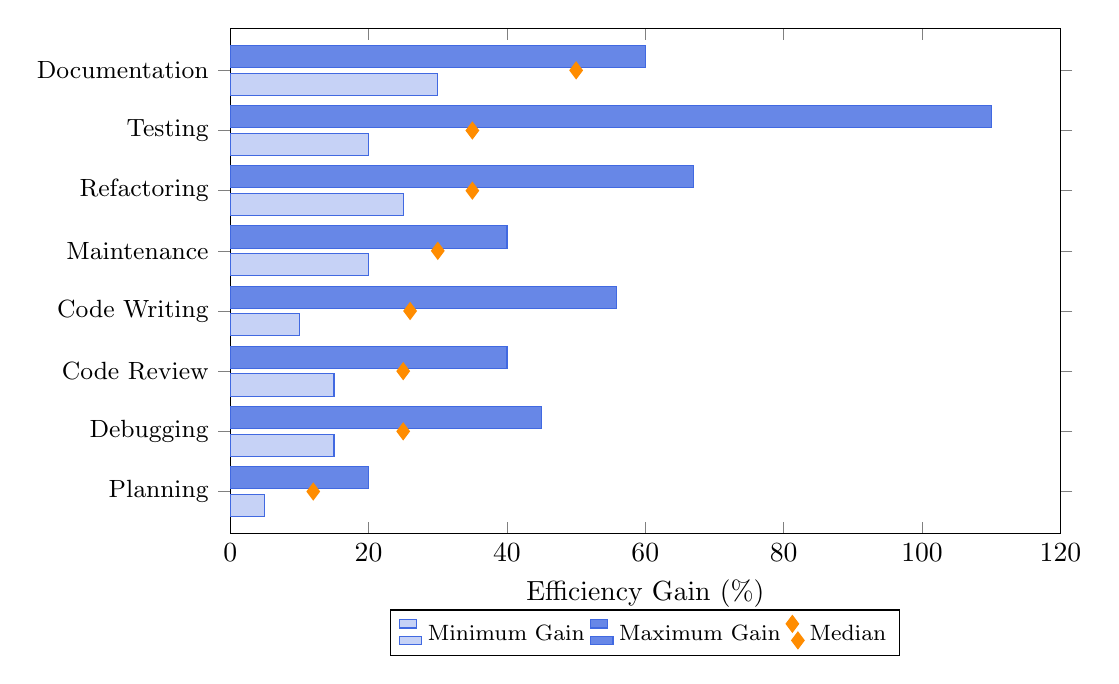
\begin{tikzpicture}
\begin{axis}[
    xbar,
    width=\columnwidth,
    height=8cm,
    xlabel={Efficiency Gain (\%)},
    symbolic y coords={Planning, Debugging, Code Review, Code Writing, Maintenance, Refactoring, Testing, Documentation},
    ytick=data,
    yticklabel style={font=\small},
    xmin=0,
    xmax=120,
    bar width=8pt,
    legend style={at={(0.5,-0.15)}, anchor=north, legend columns=3, font=\footnotesize},
    legend cell align={left},
    nodes near coords style={font=\tiny},
    enlarge y limits=0.1,
]

% Min values (lighter shade)
\addplot[fill=chartblue!30, draw=chartblue] coordinates {
    (5,Planning)
    (15,Debugging)
    (15,Code Review)
    (10,Code Writing)
    (20,Maintenance)
    (25,Refactoring)
    (20,Testing)
    (30,Documentation)
};

% Max values (darker shade)
\addplot[fill=chartblue!80, draw=chartblue] coordinates {
    (20,Planning)
    (45,Debugging)
    (40,Code Review)
    (55.8,Code Writing)
    (40,Maintenance)
    (67,Refactoring)
    (110,Testing)
    (60,Documentation)
};

% Median markers
\addplot[only marks, mark=diamond*, mark size=3pt, fill=chartorange, draw=chartorange] coordinates {
    (12,Planning)
    (25,Debugging)
    (25,Code Review)
    (26,Code Writing)
    (30,Maintenance)
    (35,Refactoring)
    (35,Testing)
    (50,Documentation)
};

\legend{Minimum Gain, Maximum Gain, Median}
\end{axis}
\end{tikzpicture}
\caption{AI Efficiency Gains by Task Category (Min-Max Range with Median)}
\label{fig:efficiency_gains}
\end{figure}

\subsection{Developer Time Allocation vs. AI Impact}

Figure~\ref{fig:time_vs_impact} presents a scatter plot comparing the time developers spend on various activities against the potential AI impact for each activity.

\begin{figure}[htbp]
\centering
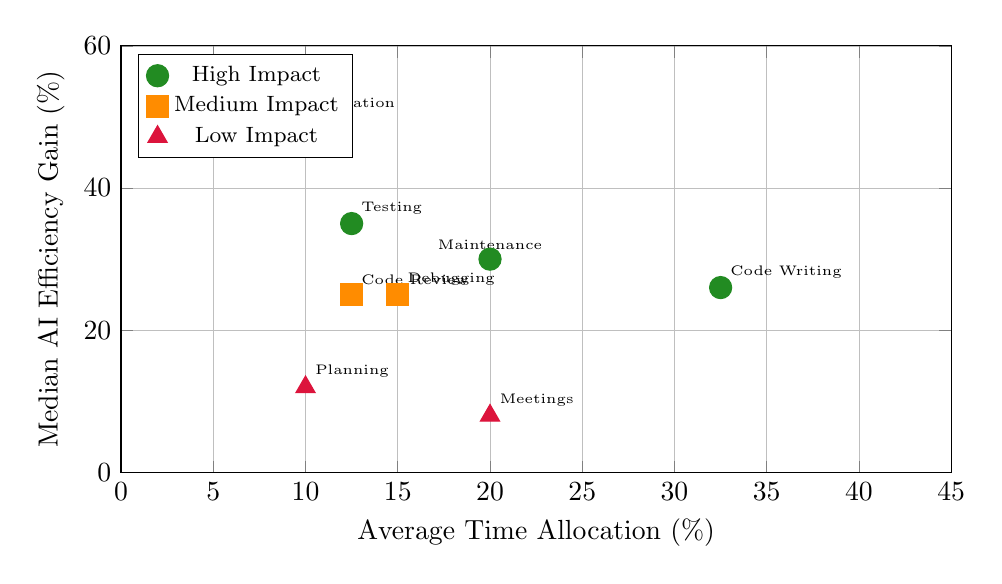
\begin{tikzpicture}
\begin{axis}[
    width=\columnwidth,
    height=7cm,
    xlabel={Average Time Allocation (\%)},
    ylabel={Median AI Efficiency Gain (\%)},
    xmin=0, xmax=45,
    ymin=0, ymax=60,
    grid=both,
    grid style={line width=.1pt, draw=gray!30},
    major grid style={line width=.2pt,draw=gray!50},
    scatter/classes={
        high={mark=*,chartgreen,mark size=4pt},
        medium={mark=square*,chartorange,mark size=4pt},
        low={mark=triangle*,chartred,mark size=4pt}
    },
    legend style={at={(0.02,0.98)}, anchor=north west, font=\footnotesize},
]

% High impact tasks
\addplot[scatter, only marks, scatter src=explicit symbolic]
coordinates {
    (32.5,26) [high]
    (12.5,35) [high]
    (7.5,50) [high]
    (20,30) [high]
};

% Medium impact tasks
\addplot[scatter, only marks, scatter src=explicit symbolic]
coordinates {
    (12.5,25) [medium]
    (15,25) [medium]
};

% Low impact tasks
\addplot[scatter, only marks, scatter src=explicit symbolic]
coordinates {
    (20,8) [low]
    (10,12) [low]
};

% Labels
\node[font=\tiny, anchor=south west] at (axis cs:32.5,26) {Code Writing};
\node[font=\tiny, anchor=south west] at (axis cs:12.5,35) {Testing};
\node[font=\tiny, anchor=south west] at (axis cs:7.5,50) {Documentation};
\node[font=\tiny, anchor=south] at (axis cs:20,30) {Maintenance};
\node[font=\tiny, anchor=south west] at (axis cs:12.5,25) {Code Review};
\node[font=\tiny, anchor=south west] at (axis cs:15,25) {Debugging};
\node[font=\tiny, anchor=south west] at (axis cs:20,8) {Meetings};
\node[font=\tiny, anchor=south west] at (axis cs:10,12) {Planning};

\legend{High Impact, Medium Impact, Low Impact}
\end{axis}
\end{tikzpicture}
\caption{Developer Time Allocation vs. AI Impact Potential}
\label{fig:time_vs_impact}
\end{figure}

\subsection{Median Efficiency Gains Summary}

Figure~\ref{fig:median_gains} presents a bar chart of median AI efficiency gains across all task categories.

\begin{figure}[htbp]
\centering
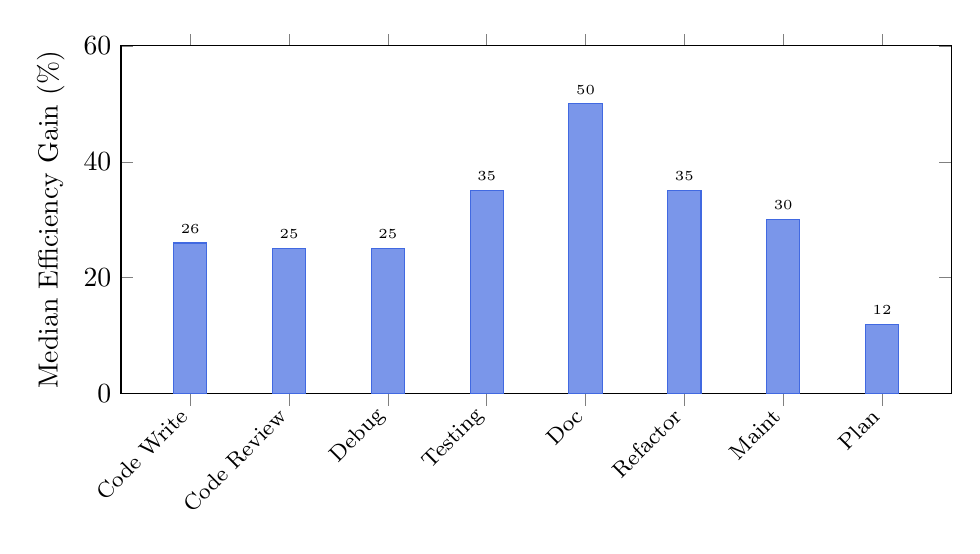
\begin{tikzpicture}
\begin{axis}[
    ybar,
    width=\columnwidth,
    height=6cm,
    ylabel={Median Efficiency Gain (\%)},
    symbolic x coords={Code Write, Code Review, Debug, Testing, Doc, Refactor, Maint, Plan},
    xtick=data,
    xticklabel style={font=\footnotesize, rotate=45, anchor=east},
    ymin=0,
    ymax=60,
    bar width=12pt,
    nodes near coords,
    nodes near coords style={font=\tiny},
    every node near coord/.append style={above},
    enlarge x limits=0.1,
]

\addplot[fill=chartblue!70, draw=chartblue] coordinates {
    (Code Write, 26)
    (Code Review, 25)
    (Debug, 25)
    (Testing, 35)
    (Doc, 50)
    (Refactor, 35)
    (Maint, 30)
    (Plan, 12)
};

\end{axis}
\end{tikzpicture}
\caption{Median AI Efficiency Gains by Task Category}
\label{fig:median_gains}
\end{figure}

\subsection{Experience Level Impact}

Figure~\ref{fig:experience} illustrates how AI efficiency gains vary by developer experience level across different task types.

\begin{figure}[htbp]
\centering
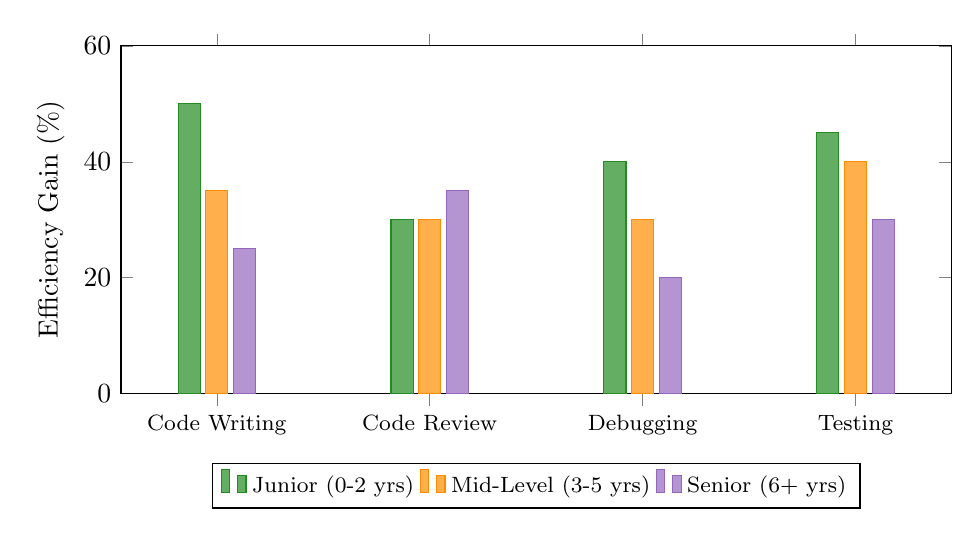
\begin{tikzpicture}
\begin{axis}[
    ybar,
    width=\columnwidth,
    height=6cm,
    ylabel={Efficiency Gain (\%)},
    symbolic x coords={Code Writing, Code Review, Debugging, Testing},
    xtick=data,
    xticklabel style={font=\footnotesize},
    ymin=0,
    ymax=60,
    bar width=8pt,
    legend style={at={(0.5,-0.2)}, anchor=north, legend columns=3, font=\footnotesize},
    enlarge x limits=0.15,
]

% Junior
\addplot[fill=chartgreen!70, draw=chartgreen] coordinates {
    (Code Writing, 50)
    (Code Review, 30)
    (Debugging, 40)
    (Testing, 45)
};

% Mid-Level
\addplot[fill=chartorange!70, draw=chartorange] coordinates {
    (Code Writing, 35)
    (Code Review, 30)
    (Debugging, 30)
    (Testing, 40)
};

% Senior
\addplot[fill=chartpurple!70, draw=chartpurple] coordinates {
    (Code Writing, 25)
    (Code Review, 35)
    (Debugging, 20)
    (Testing, 30)
};

\legend{Junior (0-2 yrs), Mid-Level (3-5 yrs), Senior (6+ yrs)}
\end{axis}
\end{tikzpicture}
\caption{AI Efficiency Gains by Developer Experience Level}
\label{fig:experience}
\end{figure}

\section{Discussion}

\subsection{Implications for Practice}

The evidence synthesized in this review suggests several important implications for software engineering practice:

\textbf{Targeted Tool Deployment:} Organizations should prioritize AI tool deployment for tasks showing the highest efficiency gains, particularly code generation, documentation, and testing. The wide variance in gains suggests that context-specific evaluation is essential before broad deployment.

\textbf{Training and Enablement:} Research indicates that efficiency gains require proper training. Microsoft research finds that it can take 11 weeks for users to fully realize the satisfaction and productivity gains of using AI tools \cite{github2024}. Organizations should invest in structured enablement programs.

\textbf{Quality Assurance Integration:} While AI accelerates many tasks, human oversight remains critical. The research consistently shows that AI suggestions require verification, and over-reliance can introduce new quality issues.

\subsection{Limitations and Future Research}

Several limitations affect the current body of research:

\begin{enumerate}
    \item Many studies use controlled laboratory settings that may not reflect real-world development complexity
    \item Self-reported productivity measures may be subject to bias
    \item The rapid evolution of AI tools means findings may become outdated quickly
    \item Limited research exists on long-term effects and learning curves
\end{enumerate}

Future research should focus on longitudinal studies examining sustained productivity impacts, investigation of team-level effects beyond individual productivity, and development of standardized metrics for AI-assisted development evaluation.

\section{Conclusion}

This comprehensive review synthesizes evidence from IEEE, ACM, and other peer-reviewed sources to quantify the impact of AI on software engineering daily tasks. The findings demonstrate that AI tools can provide efficiency gains ranging from 10\% to over 100\% depending on the task type, with median improvements of 25-50\% across most activities.

Code generation and documentation show the most consistent benefits, while debugging and planning present more variable results dependent on context and complexity. The variance between minimum and maximum gains highlights the importance of organizational factors, developer experience, and implementation quality in realizing AI's productivity potential.

As AI capabilities continue to advance, software engineering practice will likely undergo significant transformation. Organizations that strategically deploy AI tools while maintaining appropriate human oversight will be best positioned to capture efficiency gains while maintaining software quality and team effectiveness.

\bibliographystyle{plain}

\begin{thebibliography}{14}

\bibitem{meyer2019}
A.~N. Meyer, T.~Fritz, G.~C. Murphy, and T.~Zimmermann, ``Today was a Good Day: The Daily Life of Software Developers,'' \textit{IEEE Transactions on Software Engineering}, vol.~47, no.~5, pp.~1028--1047, 2021.

\bibitem{peng2023}
S.~Peng, E.~Kalliamvakou, P.~Cihon, and M.~Demirer, ``The Impact of AI on Developer Productivity: Evidence from GitHub Copilot,'' \textit{arXiv preprint arXiv:2302.06590}, 2023.

\bibitem{sadowski2018}
C.~Sadowski, E.~S{\"o}derberg, L.~Church, M.~Sipko, and A.~Bacchelli, ``Modern Code Review: A Case Study at Google,'' in \textit{Proc. 40th Int. Conf. Software Engineering: Software Engineering in Practice (ICSE-SEIP)}, ACM, 2018, pp.~181--190.

\bibitem{smit2024}
D.~Smit, H.~Smuts, P.~Louw, J.~Pielmeier, and C.~Eidelloth, ``The impact of GitHub Copilot on developer productivity from a software engineering body of knowledge perspective,'' in \textit{AMCIS 2024 Proceedings}, 2024.

\bibitem{acm2024}
M.~Vijayvergiya \textit{et al.}, ``AI-Assisted Assessment of Coding Practices in Modern Code Review,'' in \textit{Proc. 1st ACM Int. Conf. AI-Powered Software}, 2024, pp.~85--93.

\bibitem{mckinsey2023}
McKinsey \& Company, ``Unleash developer productivity with generative AI,'' \textit{McKinsey Digital Insights}, June 2023.

\bibitem{dora2024}
DORA Research Team, ``2024 DORA Report: Accelerate State of DevOps,'' Google Cloud, 2024.

\bibitem{smite2021}
D.~{\v{S}}mite, A.~Tkalich, N.~B. Moe, E.~Klotins, and M.~P. Buvik, ``Changes in perceived productivity of software engineers during COVID-19 pandemic: The voice of evidence,'' \textit{Journal of Systems and Software}, vol.~182, p.~111083, 2021.

\bibitem{forsgren2021}
N.~Forsgren, M.~A. Storey, C.~Maddila, T.~Zimmermann, B.~Houck, and J.~Butler, ``The SPACE of Developer Productivity,'' \textit{ACM Queue}, vol.~19, no.~1, pp.~20--48, 2021.

\bibitem{github2024}
GitHub, ``Measuring Impact of GitHub Copilot,'' GitHub Resources, 2024. [Online]. Available: \url{https://resources.github.com/copilot/}

\bibitem{llm4fin2024}
LLM4Fin Research Team, ``LLM4Fin: Fully Automating LLM-Powered Test Case Generation for FinTech Software Acceptance Testing,'' in \textit{Proc. ISSTA 2024}, 2024.

\bibitem{meta2024}
Meta AI Research, ``Automated Unit Test Improvement using Large Language Models at Meta,'' 2024.

\bibitem{linearb2024}
LinearB, ``Gen AI Research: Software Development Productivity At Google,'' LinearB Blog, 2024.

\bibitem{microsoft2025}
Microsoft Research, ``Debug-gym: An Environment for AI Coding Tools to Learn How to Debug Code Like Programmers,'' Microsoft Research Blog, 2025.

\bibitem{metr2025}
METR, ``Measuring the Impact of Early-2025 AI on Experienced Open-Source Developer Productivity,'' METR Technical Report, 2025.

\bibitem{index2025}
Index.dev, ``Developer Productivity Statistics with AI Tools 2025,'' Index.dev Research, 2025.

\bibitem{bain2024}
Bain \& Company, ``Beyond Code Generation: More Efficient Software Development,'' \textit{Technology Report 2024}, 2024.

\end{thebibliography}

\end{document}
